\chapter{Evaluation: Container-Runtimes}
\label{chap:compCtnrRuntimes}

Container-Runtimes sind das Herz eines jeden Container-Angebots. Sie instanziieren übergebene Prozesse in isolierten Containern. In diesem Kapitel werden verschiedene Runtimes miteinander verglichen und veranschaulicht, wie Runtimes andere neben Docker für spezielle Anforderungen besser geeignet sind.

\section{Vorgehen}
\label{sec:vorgehen}
Um verschiedene Runtimes zu vergleichen wurde eine eigene Anwendung mit drei Microservices implementiert. Dabei wurden, wie in \fref{fig:todosStack} zu sehen, verschiedene Technologien verwendet, um zu prüfen, wie die getesteten Container-Runtimes mit diesen umgehen. Diese wurde im Folgenden mit verschiedenen Runtimes lokal bereitgestellt.

\begin{figure}[h]
	\begin{center}
		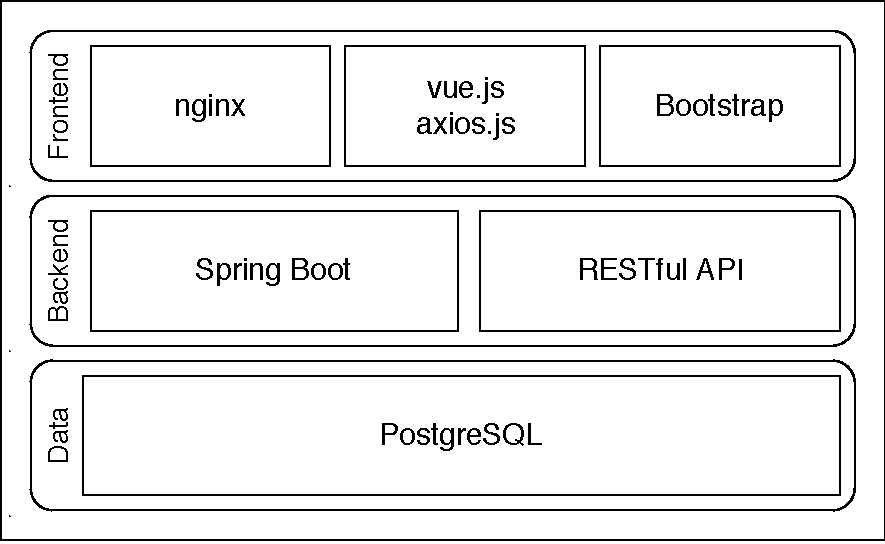
\includegraphics[width=0.65\textwidth]{bilder/microservice-example-stack.pdf}
		\caption{Beispielhafte Darstellung einer Micorservice-Architektur}
		\label{fig:todosStack}
	\end{center}
\end{figure}

\section{Docker Stack}
\label{sec:compDocker}
Docker ist der de facto Standard unter den Container-Technologien und bietet eine vollständige Plattform zur Verwaltung und Orchestrierung von Container (Docker Swarm), der Verbreitung von \glspl{gls-image} (Docker Hub bzw. Docker Store) und der Verwaltung des Container-Lifecycles (Docker CLI) an.


Dabei kommen innerhalb des Docker Stacks die Runtimes \texttt{runC} und \texttt{containerd} zum Einsatz. Durch die in \fref{fig:dockerStack} gezeigte Abkapselung der Runtime kann Docker auf jede beliebige \gls{acr-oci}-konforme Runtime aufbauen.

\begin{figure}[h]
	\begin{center}
		\includegraphics[width=0.9\textwidth]{bilder/docker-stack-containerd-runC.pdf}
		\caption{Docker Stack \citep{RktVsOtherProjects}}
		\label{fig:dockerStack}		
	\end{center}
\end{figure}

Der dadurch gewonnene Vorteil der Kompatibilität und Plattformunabhängigkeit bietet allerdings auch Nachteile. Falls einer der vielen Komponenten im Container-Stack einen Bug aufweist, ist das Debugging der Anwendung deutlich komplexer und Fehler können langsamer gefunden werden. Zudem benötigt der Docker-Daemon privilegierte Berechtigungen um die in \fref{sec:funktionsweise} beschriebenen Konzepte zu Nutzen. Da der Daemon auch für den Download und Bau-Prozess der Images zuständig ist, werden alle Images in Docker im Kontext des Users \texttt{root} erstellt.

\subsection{Vorgehensweise}
\label{sec:compDockerVorgehen}

Um den beispielhaften Microservice aus \fref{fig:todosStack} zu Container wurde zuerst für jeden Service ein Image erstellt und diese dann in Containern gestartet. Um dieses Vorgehen zu erleichtern wurde danach das Tool Docker Compose genutzt, um alle Container in einer Datei zu spezifizieren. Folgend werden beide Wege genauer beschrieben und Vor- bzw. Nachteile dieser Vorgehensweisen aufgezeigt.

Docker verwendet zur Beschreibung eines Images das Dockerfile. Dieses verwendet spezifische Keywords, um Docker beim Bau eines Images zu steuern (siehe \fref{lst:dockerfileExmpl}).

\begin{listing}[h]
	\begin{minted}[breaklines]{dockerfile}
FROM nginx:1.13-alpine
VOLUME /tmp
ADD ./index.html /usr/share/nginx/html/index.html
EXPOSE 80
ENTRYPOINT ["nginx","-g","daemon off"]
	\end{minted}
	\caption{Beispiel für ein Dockerfile}
	\label{lst:dockerfileExmpl}
\end{listing}

Dabei wird deklariert, von welchen Baseimage das neue Image erzeugt werden soll (\textbf{FROM}), welche Änderungen an diesem Image vorgenommen werden müssen (\textbf{VOLUME, ADD, EXPOSE}) und welchen Prozess der Container isolieren soll (\textbf{ENTRYPOINT}). Dieses Vorgehen erlaubt es einfach, neue Container auf Basis andere zu erzeugen und diese für Dritte zu Verfügung zu stellen. Zu diesem Zweck bietet Docker den Docker Hub an, der als Standardrepository im Docker Stack verwendet wird. Dieser hostet mittlerweile mehr als 100 offizielle und über 100000 Images, die aus der wachsenden Docker Community kommen. Um die in \fref{fig:todosStack} gezeigte Anwendung zu Containern benötigt man somit drei Dockerfiles. Nach dem anlegen der Dockerfiles kann mit dem Befehl \mintinline[breaklines]{bash}{docker build -t <name of image>:<tag> <path to dockerfile>} das entsprechende Image erstellt werden. Diese Images können mit \mintinline[breaklines]{bash}{docker run <name of image>:<tag>} isoliert werden. Durch diesen Prozess kann die gesamte in \fref{fig:todosStack} gezeigte Anwendung in wenigen Minuten gestartet werden.

Vereinfacht wird dieser Prozess mit dem Tool Docker Compose. Dieses erlaubt es in einer \gls{acr-yml}-Datei alle benötigten Container Images zu spezifizieren und mit dem Befehl \mintinline{bash}{docker-compose up} zu starten (siehe \fref{lst:dockerComposeTodos}).

\begin{listing}[h]
	\begin{minted}[breaklines]{yaml}
version: '3'
services:
 data:
  image: library/postgres
  environment:
   POSTGRES_USER: docker
   POSTGRES_PASSWORD: docker
   POSTGRES_DB: todos
 back:
  build:
   context: ./backend
   ports:
    - "8080:8080"
   environment:
    POSTGRES_PORT: 5432
    POSTGRES_IP: data
 front:
  image: nginx:latest
  ports:
   - "80:80"
  volumes:
   - ./frontend:/usr/share/nginx/html
	\end{minted}
	\caption{docker-compose.yaml für Micorservices}
	\label{lst:dockerComposeTodos}
\end{listing}

Der größte Unterschied liegt dabei in der Art und Weise, wie Container innerhalb des Compose-Clusters angesprochen werden können. Jeder Container bekommt zu seiner IP einen DNS Eintrag mit dem Namen des Service im docker-compose.yml. Dadurch lassen sich die Services einfacher miteinander verknüpfen, da die IP des Containers nicht bekannt sein muss.

\subsection{Bewertung}
\label{sec:compDockerBewertung}
Docker erlaubt es die Anwendung einfach in Containern bereitzustellen. Dafür ist vor allem die große Auswahl bereits bestehender Images verantwortlich, aber auch die einfache Nutzung durch Docker Compose. Das Format für Dockerfiles ist zwar einfach, aber grade für Unixsysteme ungewöhnlich und nur mit Dokumentation nutzbar. Die Vorteile der einfachen Nutzung kommen allerdings zu einem Preis: Sicherheit. Images auf dem Dockerhub sind nicht verifizierbar, können somit Schadware und Sicherheitsprobleme mit sich bringen. Zudem baut Docker jedes Image unter dem Nutzer root, wodurch potentielle Sicherheitsrisiken, wie falsch konfigurierte AppArmor Profile, nicht beim Bau-Prozess auffallen. Viele dieser Probleme kommen durch die in \fref{fig:dockerStack} gezeigte Architektur, bei der die Docker-\gls{acr-cli} nur ein Client ist, der den Docker Daemon steuert. Diese Herangehensweise erlaubt keine Integration mit bereits vorhandenen Linux Tools wie \texttt{systemd} oder \texttt{upstart}.

Ein weiterer Nachteil gegenüber anderen Runtimes ist die Pflicht eines Image-Repositories. Um Docker Images zu teilen und zu verbreiten wird ein solches Zwanghaft benötigt und muss somit gehostet, gewartet und konfiguriert werden. Um diese Aufgaben zu erleichtern bieten Google, Amazon, CoreOS und weitere gehostete Container Image-Repository an.

\section{rkt}
\label{sec:compRkt}

CoreOS veröffentlicht mit rkt den aktuell größten Konkurrenten zu Docker. Dieser setzt, wie in \fref{fig:rktProcessModell} zu sehen, auf ein deutlich vereinfachtes Prozessmodell. Dieses ist linuxartiger, wodurch rkt im Vergleich zu Docker sicherer ist. Zudem ist rkt auf die Integration mit anderen Linux Tools wie \texttt{systemd} konzipiert, wodurch sich der Container überwachen und steuern lässt.

\begin{figure}[h]
	\begin{center}
		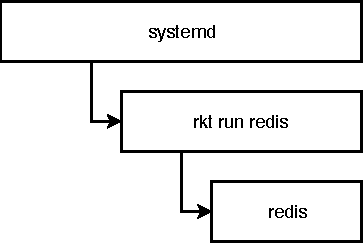
\includegraphics[scale=0.9]{bilder/rkt-process.pdf}
		\caption{rkt Prozess Modell \citep{RktVsOtherProjects}}
		\label{fig:rktProcessModell}		
	\end{center}
\end{figure}


\subsection{Vorgehensweise}
\label{sec:compRktVorgehen}

Im Gegensatz zu Docker bietet rkt die Möglichkeit verschiedene Imageformate zu nutzen um Container zu erstellen. Neben dem Dockerformat können auch OCI-konforme Bundles und \glspl{acr-aci} ausgeführt werden. Um den beispielhaften Microservice aus \fref{fig:todosStack} bereitzustellen, wurde für jeden Service ein \gls{acr-aci} erstellt. Zu diesem Zweck wird das Tool \texttt{acbuild} benötigt, welches ähnlich dem Syntax eines Dockerfiles einzelne Befehle hat um das zu erstellende \gls{acr-aci} zu spezifizieren (siehe \fref{lst:acbuildCommands}).

\begin{listing}[h]
	\begin{minted}[breaklines]{bash}
acbuild --debug begin
acbuild --debug set-name example.com/nginx
acbuild --debug dep add quay.io/coreos/alpine-sh
acbuild --debug run apk update
acbuild --debug run apk add nginx
acbuild --debug port add http tcp 80
acbuild --debug mount add html /usr/share/nginx/html
acbuild --debug set-exec -- /usr/sbin/nginx -g "daemon off;"
acbuild --debug write --overwrite nginx-latest-linux-amd64.aci
	\end{minted}
	\caption{Bash Script um \gls{acr-aci} mit \texttt{acbuild} zu erstellen \citep{AppContainer}}
	\label{lst:acbuildCommands}
\end{listing}

Ein Container mit dem daraus resultierenden \gls{acr-aci} kann mit dem Befehl \mintinline[breaklines]{bash}{systemd-run rkt run --insecure-options=image nginx-latest-linux-amd64.aci} gestartet werden. Dabei fallen folgende Unterschiede zur Herangehensweise mit Docker auf:
\begin{enumerate}
	\item \texttt{systemd-run} \\ 
	Dieses Prefix wird benötigt um einen rkt Container im Hintergrund auszuführen, vergleichbar mit \texttt{docker run -d <image>}. Da rkt kein Daemon nutzt (siehe \fref{fig:rktProcessModell}), kann es mit bekannten und verbreiteten Linux Tools genutzt werden kann. Um den Container-Prozess zu überwachen und zu steuern wird das Initsystem \texttt{systemd} verwendet.
	\item \texttt{--insecure-options=image} \\
	rkt verlangt bei jedem Image, dass es von einer vertrauenswürdigen Quelle gebaut wurde. Dazu nimmt rkt an, dass jedes Image digital signiert ist. Da dies bei dem angelegten \gls{acr-aci} nicht der Fall ist, kann dieses Verhalten mit der gegebenen Option ausgeschaltet werden.
\end{enumerate}

Um Container miteinander zu verknüpfen nutzt rkt das von der \gls{acr-cncf} publizierte \gls{acr-cni}. Dieses erlaubt es, mittels einer JSON-Konfiguration, neue Routen für den Traffic zum Container zu spezifizieren (siehe \fref{lst:cniConfig}). Dadurch kann man, ähnlich wie bei Docker Compose, einzelnen Containern DNS Namen zuweisen und somit ohne das wissen der IP Container verknüpfen.

\begin{listing}[h]
	\begin{minted}[breaklines]{json}
{
	"cniVersion": "0.2.0",
	"name": "mynet",
	"type": "bridge",
	"bridge": "cni0",
	"isGateway": true,
	"ipam": {
		"type": "host-local",
		"subnet": "10.22.0.0/16",
		"routes": [{ "dst": "0.0.0.0/0" }]
	}
}
	\end{minted}
	\caption{Beispielhafte \gls{acr-cni}-Konfiguration}
	\label{lst:cniConfig}
\end{listing}

\subsection{Bewertung}
\label{sec:compRktBewertung}
In vielen Punkten gleichen sich rkt und Docker. Bei beiden steht das Bereitstellen einer Anwendung im Mittelpunkt. Doch gerade was das Thema Sicherheit und die Linuxähnlichkeit angeht treffen unterschiedliche Ansätze aufeinander. CoreOS bewegt sich näher an dem für Linuxsysteme typischen Aufbau und bietet mit rkt Integrationen zu weitverbreiteten Tools wie \texttt{systemd} an. Zudem benötigt rkt keine privilegierten Berechtigungen und arbeitet vollständig im Nutzerkontext. Durch dieses Vorgehen ist eine Privilege-Escalation weniger wahrscheinlich. rkt lässt sich zudem granularer Steuern, da keinen Daemon genutzt wird. Diese Vorteile kommen allerdings zum Preis von mehr Konfigurationsaufwand. Wenn man \fref{lst:dockerfileExmpl} und \fref{lst:acbuildCommands} vergleicht wird man feststellen, dass das Erstellen von Images mit \texttt{acbuild} komplexer und aufwändiger ist. Zudem wird neben rkt das Tool \texttt{acbuild} benötigt, da rkt selber keine Images erstellen kann, sondern lediglich eine Runtime bietet. Weiterreichend ist die Konfiguration des Netzwerks mittels \gls{acr-cni} umfangreicher aber auch komplexer.

Ein großer Vorteil gegenüber Docker ist die Art und Weise, wie man Images teilen und verbreiten kann. Für \glspl{acr-aci} ist kein private gehostetes Imagerepository notwendig, wie bei Docker. Es reicht lediglich ein Webserver und einige Metatags in der index.html (siehe \fref{lst:rktReposHTML}). Dadruch entfällt der Konfigurationsaufwand, der mit dem Hosten eines Repositories anfällt.

\begin{listing}
	\begin{minted}[breaklines, breakafter=/]{html}
<!DOCTYPE html>
<html lang="en">
	<head>
		<meta charset="utf-8">
		<meta name="ac-discovery" content="example.com/hello https://example.com/images/{name}-{version}-{os}-{arch}.{ext}">
		<meta name="ac-discovery-pubkeys" content="example.com/hello https://example.com/pubkeys.gpg">
	</head>
</html>
	\end{minted}
	\caption{index.html mit Metatags um \glspl{acr-aci} bereitzustellen}
	\label{lst:rktReposHTML}
\end{listing}

\pagebreak

\section{LXD / LXC}
\label{sec:compLXD}

2008 kam mit LXC die erste vollwertige Implementierung einer Container-Runtime auf den Markt. Diese erlaubte es, ohne Veränderung des Kernels, Prozesse zu isolieren. 2015 wurde mit LXD eine Erweiterung von LXC veröffentlicht, die zu LXC eine RESTful API anbietet. Im Gegensatz zu Docker und rkt ist LXD dazu gedacht, komplette Betriebssysteme in Containern bereitzustellen und nicht einzelne Applikationen. Dadurch sieht sich LXD nicht als direkte Konkurrenz zu Docker, sondern als komplementäre Technologie um mehr Sicherheit und Virtualisierung zu bieten \citep{TheLXDContainerHypervisor} (siehe \fref{fig:cloudStack}).

\begin{figure}[h]
	\begin{center}
		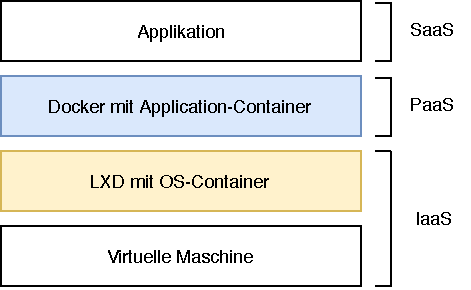
\includegraphics[]{bilder/cloud-stack.pdf}
		\caption{Docker Container in LXD Container}
		\label{fig:cloudStack}		
	\end{center}
\end{figure}

\subsection{Vorgehensweise}
\label{sec:compLXDVorgehen}

Auch wenn LXD nicht hauptsächlich dafür gedacht ist, Applikationen und Services bereitzustellen, ist es möglich, diese mit LXD zu isolieren. Im Gegensatz zu Docker oder rkt können mit LXD mehrere Prozesse in einem Container isoliert werden. Um den in \fref{fig:todosStack} gezeigten Service mit LXD bereitzustellen, muss ein Baseimage ausgewählt, die benötigten Bibliotheken, Tools und Laufzeitumgebungen installiert und die erstellten Executables in das Dateisystem des Containers kopiert werden. Dazu kann man die mit LXD mitgelieferte CLI lxc nutzen (siehe \fref{lst:lxdConfig}).

\begin{listing}[h]
	\begin{minted}[breaklines]{bash}
lxc launch ubuntu:16.04 todos
lxc file push /service/frontend/index.html /usr/share/nginx/html
lxc file push /service/backend/target/todos-backend-0.0.1-SNAPSHOT.jar /home/app.jar
lxc exec todos -- /bin/bash
# install and configure environment tools
# execute postgres, app.jar and nginx
exit
	\end{minted}
	\caption{Shellbefehle um LXD Container zu starten}
	\label{lst:lxdConfig}
\end{listing}

Durch dieses Vorgehen ist die Anwendung vollständig isoliert vom Hostsystem, allerdings von außen nicht aufrufbar, da LXD keine Änderungen am Netzwerk des Hostsystems vornimmt. Um einen Container von außen zugänglich zu machen muss zusätzlich eine EthernetBridge auf dem Hostsystem konfiguriert und mit dem Container verknüpft werden.

\subsection{Bewertung}
\label{sec:compLXDBewertung}
Wie man an \fref{lst:lxdConfig} erkennt, erwartet LXD Wissen über die Bedienung von Linuxsystemen. Vor allem die Konfiguration des Containernetzwerks ist komplexer als bei Docker oder rkt. Da LXD für die Isolation von Betriebssystemen gedacht ist, gibt es keine Images für Runtimes oder \gls{acr-saas}-Angebote, sondern Images für einzelne Betriebssysteme wie Alpine Linux oder Debian. Der Fokus liegt dabei allerdings auf Ubuntu, das wie LXD auch von Canonical angeboten wird. Die \gls{acr-ipc} ist gestaltet sich bei LXD deutlich leichter durch den Vorteil, dass mehrere Prozesse in einem Container isoliert werden können. Allerdings ist das Anbinden des Container an das Netzwerk des Hosts komplexer als bei Applikation Containern. LXD bietet hierfür keine automatische Konfiguration, wodurch Linux Know-How benötigt wird. Zudem hat das isolieren der Services in einzelne Container den Vorteil, das gezielt die Aspekte der Anwendung skaliert werden können, die unter Last stehen.

Der größte Vorteil von LXD gegenüber Docker oder rkt ist die REST-API. Diese erlaubt es, ohne Zugriff auf das Hostsystem Container zu steuern, Checkpoints zu erstellen und die Last eines Containers zu überwachen. Für diesen Zweck wird bei Docker ein Third-Party Orchestrirungstool, wie z.B. \gls{acr-k8} benötigt.

\section{runC}
\label{sec:comprunC}

Wie in \fref{sec:standards} beschrieben ist das Interesse für einen Standard im Container-Umfeld so groß wie nie. Aus diesem Grund haben sich die meisten Firmen in der \gls{acr-oci} zusammengeschlossen und mit \texttt{runC} eine Implementierung des definierten Standards veröffentlicht. Diese findet bereits innerhalb Dockers (siehe \fref{fig:dockerStack}), wie auch bei \gls{acr-k8} in Form von \texttt{cri-o}.

\subsection{Vorgehensweise}
\label{sec:comprunCVorgehen}

Im Gegensatz zu Docker, rkt oder LXD nutzt runC keine Images um einen Container zu spezifizieren, sondern ein Bundle bestehend aus 2 Dateien:
\begin{itemize}
	\item rootfs.tar \\
	runC benötigt ein Verzeichnis, welches als Baseimage verwendet wird.
	\item config.json \\
	Konfiguration im JSON Format, die beschreibt, wie der Prozess innerhalb des rootfs ausgeführt werden soll.
\end{itemize}

Wie ein \texttt{rootfs.tar}-Archiv erstellt werden kann wurde bereit in \fref{sec:tarball} beschrieben. Eine weitere Möglichkeit ist das exportieren aus Docker (siehe \fref{lst:dockerExport})

\begin{listing}[h]
	\begin{minted}[breaklines]{bash}
docker export \$(docker create -v /service/frontend:/usr/share/nginx/html nginx) | tar -C rootfs -xvf -
	\end{minted}
	\caption{Exportieren eines \texttt{rootfs} aus Docker Container}
	\label{lst:dockerExport}
\end{listing}

Um einen Container mit runC zu starten wird zusätzlich eine config.json benötigt. Diese kann mit \mintinline{bash}{runC spec} erzeugt werden. Die dadurch erstellte Datei beinhaltet eine vorgegebene Spezifikation, die in \fref{lst:configJSON} auszugsweise zu sehen ist. Beim Start eines Containers mit der gegebenen Konfiguration wird eine isolierte Shell gestartet. Um einen anderen Prozess, beispielsweise nginx zu starten muss ein entsprechendes rootfs erstellt und in der Konfiguration die Schlüssel \mintinline{json}{{"args": ["sh"]}} und \mintinline{json}{{"process": {"terminal": true,}}} geändert werden. Dadurch ist es auch möglich, entkoppelte Container zu starten, vergleichbar mit dem Docker-\gls{acr-cli}-Argument \texttt{-d}. 

\newpage

\begin{listing}[H]
	\begin{minted}[breaklines, breakafter=/]{json}
{
	"ociVersion": "1.0.0",
	"process": {
		"terminal": true,
	"user": {
		"uid": 0,
		"gid": 0
	},
	"args": [
		"sh"
	],
	"env": [
		"PATH=/usr/local/sbin:/usr/local/bin:/usr/sbin:/usr/bin:/sbin:/bin",
		"TERM=xterm"
	],
	"cwd": "/",
	"capabilities": {
		"bounding": [
			"CAP_AUDIT_WRITE",
		],
	},
	"root": {
		"path": "rootfs",
		"readonly": true
	},
	"hostname": "runC",
	"mounts": [
	{
		"destination": "/proc",
		"type": "proc",
		"source": "proc"
	},
	\end{minted}
	\caption{Auszug aus Standardspezifikation durch den Aufruf von \mintinline{bash}{runC spec}}
	\label{lst:configJSON}
\end{listing}


\subsection{Bewertung}
\label{sec:comprunCBewertung}

Die \gls{acr-oci} bietet mit runC eine standardisierte Container-Runtime, die eine einfache API besitzt und von den meisten Cloud-Providern unterstützt wird. Dabei ist vor allem die Steuerung und Konfiguration durch die erstellte \texttt{config.json} einfach und verständlich. Zudem bietet runC die Möglichkeit, Container ohne root-Berechtigungen zu starten. Diese rootless Container sind deutlich sicherer, da sie die Isolation nicht durch wenige Systemcalls des Linux-Kernels umgehen können.

Neben den Vorteilen sind die Nachteile an runC als Standalone Container-Runtime allerdings groß. So werden für jeden Container zwei Dateien benötigt, die nicht von runC verwaltet werden. Außerdem bietet runC keine Repositories für bestehende Images an. Ein weiterer großer Nachteil ist das erforderliche Wissen über Linux Kernel-Funktionen wie Capabilities oder Namespaces. Im Gegensatz zu rkt unterstützt runC auch keine automatische Prüfung der Signatur \citep{RktVsOtherProjects}. 

\section{VM basierte Runtimes}
\label{sec:compVMbased}
Die Isolation durch Container kann umgangen werden und somit Zugriff auf alle weiteren Container bzw. Prozesse einer VM bis hin zu der gesamten Infrastruktur erhalten werden. Um potentiell unsicheren Code dritter auf eigenen Servern auszuführen wurden vor Containern \glspl{acr-vm} genutzt. Diese sind allerdings, wie in \fref{chap:grundlagen} erläutert, langsamer. Dieses Problem haben Firmen wie Intel, HyperHQ und Google erkannt und Lösungsvorschläge implementiert.

\subsection{Kata Containers}
\label{sec:compVMbasedKata}

Kata Containers ist eine Initiative von Intel und HyperHQ, die die Projekte Intel Clear Containers und runV zusammenlegt. Kata Containers vereint dabei die Performance von Containern und die Sicherheit von \glspl{acr-vm}. Um dies zu erreichen werden einzelne Container in einer eigenen VM gestartet und somit der Kernel für jeden Container isoliert (siehe \fref{fig:kataContainers}). Die gestarteten VMs sind dabei auf das Minimum an Funktionalität reduziert und sind somit deutlich leichtgewichtiger als vollwertige VMs.

\begin{figure}[h]
	\subfigure[Container mit z.B. Docker]{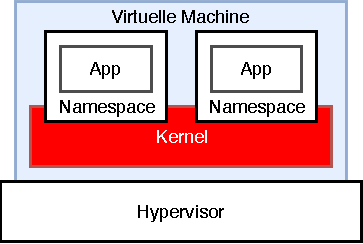
\includegraphics[width=0.49\textwidth]{bilder/container.pdf}}
	\hfill
	\subfigure[Kata Containers]{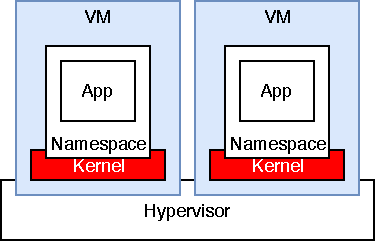
\includegraphics[width=0.49\textwidth]{bilder/kata.pdf}}
	\caption{Kata Container im Vergleich zu Docker Container}
	\label{fig:kataContainers}
\end{figure}

Vorteile dieser Herangehensweise ist die gegebene Sicherheit innerhalb eines Containers. Diese ist durch die extra Isolation mittels einer VM vergleichbar mit selbiger und somit deutlich besser als bei Containern. Der größte Nachteil ist die langsamere Startzeit und der größere Footprint, da ein Extra Agent benötigt wird um Kata Containers zu starten.

\subsection{gVisor}
\label{sec:compVMbasedGVisor}

Im Gegensatz zu Kata Containers wählt Google mit gVisor einen anderen Ansatz, welches Anfang Mai 2018 als Open Source Projekt veröffentlicht wurde \citep{OpenSourcingGVisoraSandboxedContainerRuntime}. Bei gVisor wird eine userspaced Implementation der meisten Systemaufrufe des Linux-Kernels gestellt. Diese werden alternativ zum Kernel des Hostsystems aufgerufen (siehe \fref{fig:gVisor}). Durch diese Vorgehensweise ist es gVisor möglich, sicherer als Container und schneller als VMs zu sein.

\begin{figure}[h]
	\begin{center}
		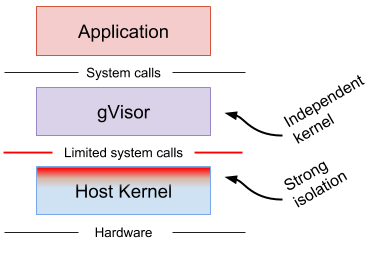
\includegraphics[scale=0.7]{bilder/gVisor.png}
		\caption{gVisor blockt Systemaufrufe zum Kernel ab \citep{OpenSourcingGVisoraSandboxedContainerRuntime}}
		\label{fig:gVisor}		
	\end{center}
\end{figure}

\pagebreak
\subsection{Bewertung}
\label{sec:compVMbasedBewertung}
Sicherheit spielt aktuell in der Cloud eine große Rolle. Angriffe wie Dirty COW im Jahr 2016 haben aufgezeigt, wie unsicher Container gegen gewissen Angriffe sein können \citep{DirtyCOWCVE20165195}. Technologien wie gVisor oder Kata Containers helfen bei der Isolation durch und bleiben dabei weiterhin skalierbar, allerdings auf Kosten der Performance.

\section{Fazit}
\label{sec:compFazit}

Die Auswahl an verschiedenen Container-Runtimes ist groß und wächst zunehmend. Dabei legen viele Runtimes seit 2015 Wert darauf, den von der \gls{acr-oci} spezifizierten Standard zu erfüllen. Dadurch ist es zunehmend einfacher möglich, eine Alternative Container-Runtime neben Docker zu wählen. Dabei bieten rkt, LXD oder auch gVisor verschiedene Vor- und Nachteile gegenüber Docker. Folgend werden die untersuchten Runtimes gegenübergestellt und eine Empfehlung für den in \fref{sec:vorgehen} geschilderten Sachverhalt gegeben. Dabei werden vor allem die folgenden Kriterien betrachtet.
\begin{itemize}
	\item Sicherheit
	\item Einfachheit der Nutzung
	\item Bereitstellen von Images
	\item Konfigurationsaufwand
\end{itemize}

\subsection{Sicherheit}
\label{sec:compFazitSec}


Wie in \fref{fig:compFazitSec} zu sehen sind die in \fref{sec:compVMbased} deutlich sicherer als andere Runtimes. Sollte es gewünscht sein, potentiell gefährliche Software von unbekannten oder nicht vertrauenswürdigen Anbietern auszuführen, sollte definitiv auf eine Lösung wie Kata Containers oder gVisor gesetzt werden.

\begin{figure}[h]
	\begin{center}
		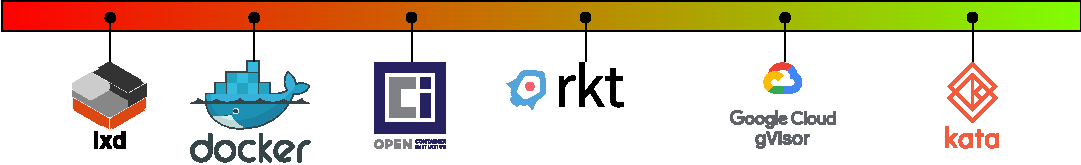
\includegraphics[width=0.9\textwidth]{bilder/rating-sec.pdf}
		\caption{Gegenüberstellung der betrachteten Runtimes auf Sicherheit}
		\label{fig:compFazitSec}
	\end{center}
\end{figure}

\subsection{Einfachheit der Nutzung}
\label{sec:compFazitEoU}

\fref{fig:compFazitEoU} zeigt die Stärke Dockers gegenüber anderen Anbietern. Durch die große Community, die Anzahl der vorhandenen Images auf der \gls{acr-saas}-Plattform Docker Hub und die gut dokumentierte API ist Docker die am einfachsten nutzbare Container-Runtime. Die \gls{acr-oci}-konformen Runtimes runC, Kata Containers und gVisor befinden sich etwa auf dem selben Level, da sie alle die selbe, standardisierte Vorgehensweise nutzen. Zum Zeitpunkt der Arbeit konnten allerdings nicht alle Services mit gVisor isoliert werden, da nicht alle benötigten Systemcalls implementiert waren. Im Zusammenspiel mit Docker hatten all diese Runtimes das selbe Level Komfort wie Docker und konnten die gleichen Images nutzen. Dies liegt an der in \fref{fig:dockerStack} gezeigten Architektur und der Austauschbarkeit von runC in dieser.

\begin{figure}[h]
	\begin{center}
		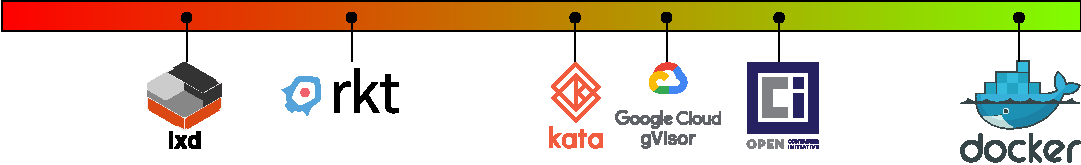
\includegraphics[width=0.9\textwidth]{bilder/rating-eou.pdf}
		\caption{Gegenüberstellung der betrachteten Runtimes auf die Einfachheit der Nutzung}
		\label{fig:compFazitEoU}
	\end{center}
\end{figure}

\subsection{Verbreiten von Images}
\label{sec:comFazitShare}

Das Bereitstellen von Images ist im Containerumfeld essentiell, um schnell Änderungen auf Cloud-Providern aufzuspielen. die Container-Runtime rkt bietet dafür die einfache Möglichkeit der Meta-Discovery, mit der es einfach fällt, Images weiterzureichen. Da der \gls{acr-oci} Standard nur wenig zur image-distribution spec aussagt ist es bislang nur schwer Möglich, ein Repository anzubieten, dass es einem ermöglichen würde, Images zu teilen. Dazu kommt bislang der Docker Hub und Tools zur Konvertierung der Docker Images zum Einsatz. LXD bietet ein Repository für verschiedene Container-Images an, allerdings ist die Auswahl der Images sehr reduziert und es gibt keine Möglichkeit, ein bereits bestehendes, verändertes Images erneut zu nutzen, wie es mit Dockerfiles der Fall ist. 

\begin{figure}[h]
	\begin{center}
		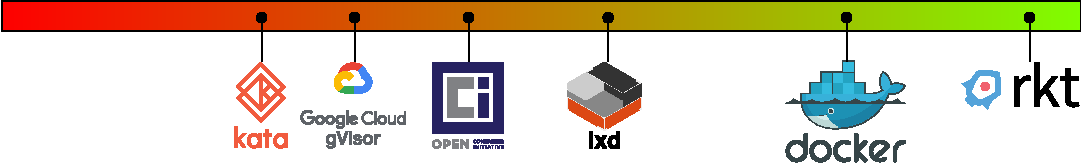
\includegraphics[width=0.9\textwidth]{bilder/rating-share.pdf}
		\caption{Gegenüberstellung der betrachteten Runtimes auf die Möglichkeit, Images zu teilen und zu verbreiten}
		\label{fig:compFazitShare}
	\end{center}
\end{figure}

\subsection{Konfigurationsaufwand}
\label{sec:compFazitConfig}

Der Konfigurationsaufwand für das betreiben der betrachteten Runtimes ist erheblich unterschiedlich. Die Installation von Docker und rkt sind dank gestellter Scripte der Hersteller deutlich leichter als es bei Kata Containers der Fall ist. Bei dieser Runtime muss zusätzlich zur Installation der CLI auch der benötigte Agent installiert und konfiguriert werden. Neben der Installation ist die Konfiguration des Containers nennenswert. Während Docker mit dem Dockerfile eine einfache Syntax zur spezifikation eines Containers besitzt, sind bei anderen Runtimes, wie z.B. LXD Linuxkentnisse notwendig. 

\begin{figure}[h]
	\begin{center}
		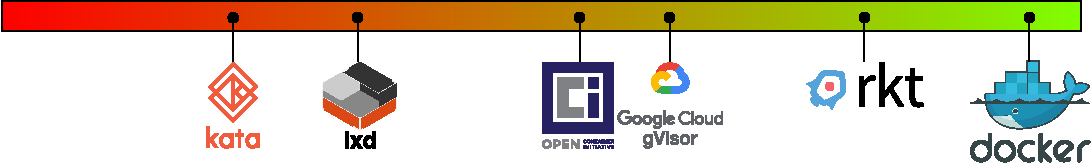
\includegraphics[width=0.9\textwidth]{bilder/rating-config.pdf}
		\caption{Gegenüberstellung der betrachteten Runtimes auf den benötigten Konfigurationsaufwand}
		\label{fig:comFazitConfig}
	\end{center}
\end{figure}

\subsection{Empfehlung}
\label{sec:compFazitEmpfehlung}

Je nach Einsatzzweck können unterschiedliche Runtimes Vorteile bieten. So sollten sicherheitsrelevante Anwendungen oder Services, bei denen man von Sicherheitslücken weiß in sichereren Runtimes, wie z.B. in Kata Containers oder gVisor, isoliert werden. Falls man eine gute Allround-Lösung für das bereitstellen einer service-orientierten Anwendung benötigt und keine sicherheitsrelevanten Daten nutzt ist Docker die vermutlich beste Lösung. Die große Anzahl bereits bestehender Images und die aktive Community sind hierbei die Hauptgründe.
